\documentclass[tikz,border=10pt]{standalone}
\usepackage{amssymb}
\usetikzlibrary{arrows.meta, bending, decorations.markings, calc, shapes.geometric}

% Definição de estilos para setas e linhas
\tikzset{
  glueArrow/.style={-{Stealth[length=3mm]}, very thick, shorten >=2pt, shorten <=2pt},
  % estilo com argumento (permite usar pathArrow=0.55, etc.)
  pathArrow/.style args={#1}{
    postaction={decorate},
    decoration={markings,
      mark=at position #1 with {\arrow[scale=1.5]{Stealth}}
    }
  },
  cycleLines/.style={very thick}
}

\begin{document}

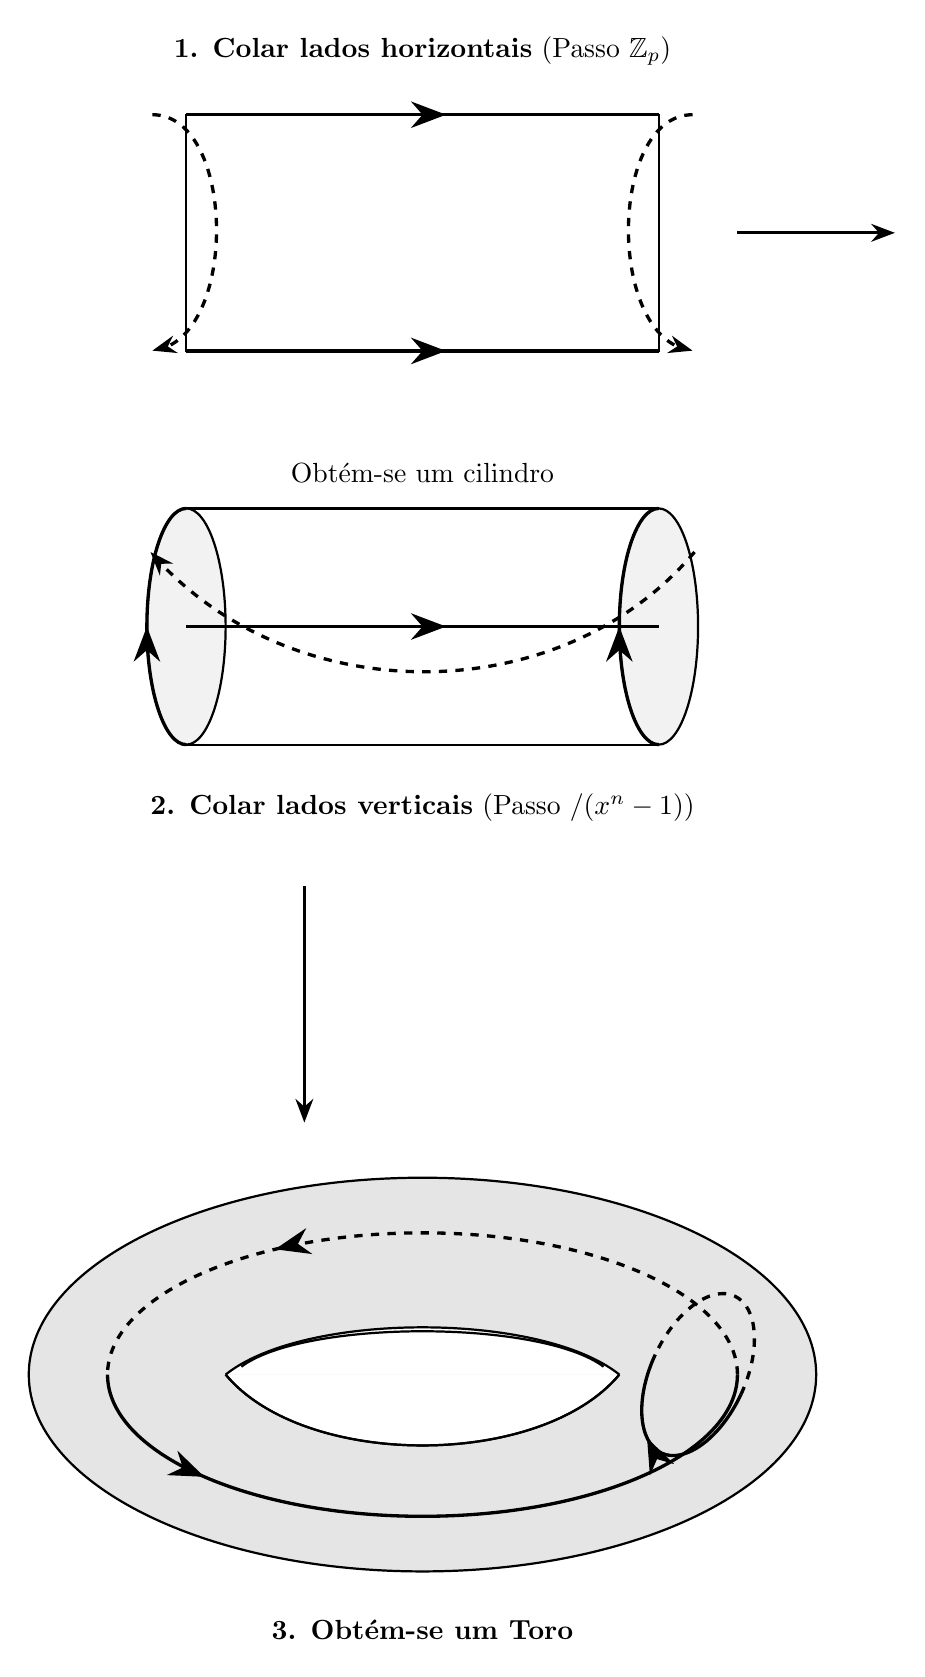
\begin{tikzpicture}
  %% --- PARTE 1: O RETÂNGULO ---
  \begin{scope}[yshift=0cm]
    % Coordenadas do retângulo
    \coordinate (A) at (0, 0);
    \coordinate (B) at (6, 0);
    \coordinate (C) at (6, 3);
    \coordinate (D) at (0, 3);

    % Desenhar o retângulo
    \draw[thick] (A) -- (B) -- (C) -- (D) -- cycle;

    % Setas indicando a colagem horizontal
    \draw[cycleLines, pathArrow=0.55] (A) -- (B);
    \draw[cycleLines, pathArrow=0.55] (D) -- (C);

    % Setas curvas indicando o movimento de colar
    \draw[glueArrow, dashed, bend left=90]  ($(D)+(-0.5,0)$) to ($(A)+(-0.5,0)$);
    \draw[glueArrow, dashed, bend right=90] ($(C)+(0.5,0)$)  to ($(B)+(0.5,0)$);

    % Texto
    \node[above] at (3, 3.5) {\textbf{1. Colar lados horizontais} (Passo $\mathbb{Z}_p$)};

    % Seta de transição para a próxima etapa
    \draw[-{Stealth[length=3mm]}, very thick] (7, 1.5) -- (9, 1.5);
  \end{scope}


  %% --- PARTE 2: O CILINDRO ---
  \begin{scope}[yshift=-5cm]
    % Desenhar o corpo do cilindro
    \draw[thick] (0, 3) -- (6, 3);
    \draw[thick] (0, 0) -- (6, 0);

    % Elipses (tampas)
    \draw[thick, fill=gray!10] (0, 1.5) ellipse (0.5 and 1.5);
    \draw[thick, fill=gray!10] (6, 1.5) ellipse (0.5 and 1.5);

    % A "costura" horizontal onde foi colado
    \draw[cycleLines, pathArrow=0.55] (0, 1.5) -- (6, 1.5);

    % Setas indicando a colagem vertical nas tampas
    \draw[cycleLines, pathArrow=0.5] (0,0) arc (270:90:0.5 and 1.5);
    \draw[cycleLines, pathArrow=0.5] (6,0) arc (270:90:0.5 and 1.5);

    % Seta curva gigante indicando o movimento de unir as pontas
    \draw[glueArrow, dashed, bend left=50] (6.5, 2.5) to (-0.5, 2.5);

    % Texto
    \node[above] at (3, 3.2) {Obtém-se um cilindro};
    \node[below] at (3, -0.5) {\textbf{2. Colar lados verticais} (Passo $/(x^n-1)$)};
  \end{scope}


  %% Seta de transição (cilindro -> toro)
  % Fora do scope pra não herdar transforms (e sem rotate)
  \draw[-{Stealth[length=3mm]}, very thick] (1.5, -6.8) -- (1.5, -9.8);


  %% --- PARTE 3: O TORO (ROSQUINHA) ---
  \begin{scope}[yshift=-13cm, xshift=3cm]
    % Contorno do toro
    \draw[thick, fill=gray!20] (0,0) ellipse (5 and 2.5);

    % Buraco central
    \begin{scope}
      \draw[thick, fill=white] (-2.5,0) .. controls (-1.5,-1.2) and (1.5,-1.2) .. (2.5,0);
      \draw[thick, fill=white] (-2.5,0) .. controls (-1.5,0.8)  and (1.5,0.8)  .. (2.5,0);
      \draw[thick] (-2.5,0) .. controls (-1.5,-1.2) and (1.5,-1.2) .. (2.5,0);
      \draw[thick] (-2.3,0.1) .. controls (-1.5,0.7)  and (1.5,0.7)  .. (2.3,0.1);
    \end{scope}

      % CICLO MENOR (Mod p)  --- corrigido: inclinação via rotação
\coordinate (mC) at (3.5,0); % centro do ciclo menor (ajuste se quiser)

\begin{scope}[rotate around={-25:(mC)}] % <-- mude o -25 para ajustar a inclinação
  % Parte da frente (contínua) — mantenho sua convenção: frente = parte de baixo
  \draw[cycleLines, pathArrow=0.6]
    ($(mC)+(0.6,0)$) arc (0:-180:0.6 and 1.1);

  % Parte de trás (tracejada)
  \draw[cycleLines, dashed]
    ($(mC)+(0.6,0)$) arc (0:180:0.6 and 1.1);
\end{scope}

    % CICLO MAIOR (Mod x^n-1)
    \draw[cycleLines, pathArrow=0.2] (-4,0) arc (180:360:4 and 1.8);
    \draw[cycleLines, dashed, pathArrow=0.7] (4,0) arc (0:180:4 and 1.8);

    % Texto final
    \node[below] at (0, -3) {\textbf{3. Obtém-se um Toro}};
  \end{scope}

\end{tikzpicture}
\end{document}
